\chapter{Introduction and Background Research}

% You can cite chapters by using '\ref{chapter1}', where the label must
% match that given in the 'label' command, as on the next line.
\label{chapter1}

% Sections and sub-sections can be declared using \section and \subsection.
% There is also a \subsubsection, but consider carefully if you really need
% so many layers of section structure.
\section{Introduction}

Algorithms such as Deep Blue \cite{CAMPBELL200257}, AlphaZero \cite{silver2018general} and more recently Player of Games\cite{schmid2021player}
have enabled computers to outsmart the smartest humans at the game of Chess.
Unfortunately all these algorithms are bound to the digital world, rendered useless when
competing against humans on a real board.  This project aims to explore a major component of this: vision.

Unlike humans, the hard part of chess for a computer is not planning which move to take next.  It is instead recognition,
localisation and manipulation of objects in 3D space which currently all present much greater challenges.
Perhaps the reason for the vision problem feeling so apparently effortless to humans is that over half of the human cortex is allocated
to visual processing \cite{snowden2012basic}.
It is also described by Szeliski as an inverse problem, and attributes that as the reason for it's difficulty
within computer science \cite{szeliski2011computer}.

Consider the vision problem for chess to be two-fold: what is the current board state and where are all of the pieces?
In particular this project will focus on the former; to produce and present a solution for determining the
state of a chess board from a video stream.  A solution reliable enough to live up to the likes of AlphaZero
in a robotic system,
but also a solution that could be immediately useful in other applications such as realtime chess analysis from a real board.

There will be a focus on deep learning techniques, with consideration for best practice, and the aim to share the
tools to more easily manage and create new datasets in this area.  Something
called for by \cite{Ding2016ChessVisionC} as a serious challenge and priority for future research.


\section{Literature Review}
\label{research}


\subsection{A \textit{Brief} History of Computer Vision}
\label{a breif history}
Computer vision is the study of making sense from visual data.  Applications include character recognition for digitising documents, segmenting and classifying
object instances for cancer screening, object tracking for sports analysis from video, and countless more.
To reach these goals, we name \textit{features} to be useful pieces of information within visual data and \textit{feature detection} to be
the class of algorithms that can extract features from visual data.

Some of the earliest work in computer vision started with Roberts from his 1965 paper \cite{roberts} describing a simple 2x2 convolutional
kernel for edge detection which soon became the predecessor to the Sobel operator in 1968 \cite{sobel}, and subsequently the still widely used
Canny edge detector developed in 1986 \cite{canny}. The ability to find edges provided a helpful backbone for detection of higher order features such as lines and corners.

Removing noise from visual data was an important preprocessing step for many algorithms.  Gaussian smoothing is the process of blurring an image with the Guassian
function and is often routinely used as a preprocessing step \cite{gaussiansmoothing}.   To note, the difference of Gaussions is also powerful technique for edge detection that is more tolerant to noise than a lot of the other
edge detectors \cite{dog}.

Another tool that is still commonly used to help more sophisticated feature extractors is \textit{thresholding}, which refers to the process of
partitioning images into two sub regions based on a pixel color/intensity threshold value.
More complex partitioning schemes are often referred to as image segmentation techniques.
Otsu's method is a famous example of an automatic global thresholding algorithm that finds a suitable threshold value for entire images without supervision,
by minimising the resulting variance, both between and within the two separated sub regions \cite{otsu}.

For higher order features more sophisticated methods are needed.  A bucket term used to describe some of these methods is \textit{template matching},
which can generally be
considered as comparing an image to known feature templates to determine if that feature is present\footnote{Neural networks perform template matching
    on an input against their learned internal features}.  The Hough transform is a common example of a higher level feature extractor, relying heavily
on edge detection, to detect lines, circles and arbitrary shapes \cite{houghtransform}.

In 1999, David Lowe invented a method that built upon the generalised hough transform and DoG's to detect more complicated features at
varying scales \cite{lowe1999object}.
This method is widely known as SIFT, or scale-invariant feature transform, and has
become a catalyst for many more approaches that follow a similar approach: RIFT (rotation-invariant feature transform) \cite{rift}, SURF (speeded up robust features) \cite{bay2006surf},
Gauss-SIFT \cite{lindeberg2015image} and many more.

\subsubsection{Neural Networks}
Fast forward to 2022 and almost all state-of-the-art computer vision solutions are built with deep learning.  A field that aims not only to solve vision but intelligence
more generally.  Deep learning is centered around artificial neural networks which roughly mimic the behavior of neurons within biological brains \cite{eluyode2013comparative}.
Arguably the first neural network applied to computer vision is the neocognitron by Kunihiko Fukushima in 1979 and was used for handwritten character recognition \cite{fukushima1982neocognitron}.
At Bell Labs Yann LeCun pushed the use of neural networks for real world vision problems forward, applying the backpropogation algorithm and differentiable convolution operators to a 
neural network like Fukushima's allowing raw images to be used as input to detect hand written digits \cite{lecun1989backpropagation}.  
This then, in 1989, is largely considered the birth of Convolutional Neural Networks (CNNs) and the beginning of the infamous MNIST dataset.  Then came another
dataset however; ImageNet.  ImageNet was the first dataset in computer vision of its size with over 11 million labelled images and 1000+ classes.  A competition was
held every year starting in 2010 \cite{deng2009imagenet}, but the best performing methods remained as classical techniques such as SIFT.
Two years later, a submission for this competition, AlexNet \cite{krizhevsky2012imagenet}, marked a breakthrough moment for CNNs beating the previous
state-of-the-art accuracy by 13\%.

CNNs have since progressively improved remaining in the number one position.  Most of these methods aimed at trying to solve the vanishing gradients problem \cite{hochreiter1998vanishing}
and overfitting with techniques like skip connections \cite{he2016deep}.
This was until the rise of transformers which signified another step change, not only for the field of computer vision but almost any field
were neural networks are useful.
Transformers doubled down on a global attention based mechanisms, dispensing with convolutions entirely \cite{vaswani2017attention}.
Originally made for the problem of machine translation in natural language processing, transformers changed the game, enabling language models such as GPT-3 \cite{radford2019language}
and BERT \cite{devlin2018bert} that have seen mainstream media attention.

\subsection{Computer Vision for Chess}
Despite chess being a very narrow application of computer vision, the amount of research effort gone into the problem of determining
board state is not insignificant.
A variety of approaches have been tried and tested, for which the following section will now summarise.

As in \cite{Ding2016ChessVisionC} the vision problem can be split into two further problems for analysis: board detection and piece recognition.

\subsubsection{Board Detection}
The problem of board detection is not specific to chess but also receives heavy research from other applications such as camera calibration \cite{cameraCalibration}.
The built in camera calibration functions in opencv \cite{opencv_library} and matlab \cite{MATLAB:2010} are used in many previous works \cite{Koray2016ACV, bowers_2014} which
provide a quick and precise solution for board detection.  However, this becomes unusable when any artifacts like chess pieces are present on the board.
This forced these authors to take the approach of an initial setup stage at inference, making the solution unfit to changes in board position during play.

Due to a chessboard's simple features many early works of line and corner point detection can be applied.  For example Hough
transforms are used to detect the lines of a chessboard \cite{CVChess, nusChessVision}.  Corner point detection methods such as the
Harris and Stephens's \cite{harris1988combined} were also common among solutions, with some authors combining approaches with further
processing such as canny edge detection to yield more reliable results \cite{irobot, CVChess, nusChessVision}.

ChESS was another corner detection algorithm that out performed the Harris and Stephen's algorithm \cite{ChESS}. This was, perhaps
interestingly, created for real-time measurement of lung function in humans, further demonstrating the attention chess board
detection has received due to its general applicability.

There are many other algorithms that require simplifications, such as custom green and red chessboards \cite{5967178, Ding2016ChessVisionC, Danner2015VisualCR}, 
multiple camera angles \cite{5967178},
or even the requirement of user input for entering the corners of the chessboard \cite{mannualcorners, irobot}.

The most impressive work came out of Poznan University of Technology, which proposes many interesting ideas that perform more
reliably in a wider range of difficult situations such as pieces being present on the board \cite{heatmap}.  They employ an iterative
approach, with each iteration containing 3 sub-tasks: line segment detection, lattice point search and chessboard position search.
In each iteration of line detection, a canny lines detector is used on many preprocessed variations of the input image
to maximize the number of relevant line detections, which are then merged using a linking function. The lattice point search starts with
the intersection of all merged lines as input, converting these intersection points to a 21x21 pixel binary image of the surrounding area and
runs them through a classifier to remove outliers.  The addition of a neural network as a classifier greatly improves
the generality of the proposed solution, as it can be resistant to lattice points that are partially covered by a chess piece.
The final sub-task then creates a heatmap over the original image, representing the likelihood of a chessboard being present.
Under the hood this is done by calculating a polyscore for the set of most likely quadrilaterals formed by the lines of the first stage,
where the polyscore is a function of the area of said quadrilateral and the number of lattice points contained within it.
It is the quadrilateral that produces the highest polyscore that is used to segment the image for input to the next iteration, until the quadrilateral
points converge.  The main disadvantage of this approach compared to others is that it can take up to 5 seconds to process one frame.
For most use cases however this will be sufficient, unless realtime board training is required.

\subsubsection{Piece Recognition}

Piece recognition has had less active research than board segmentation.  Most chess vision systems completely avoid directly classifying pieces by
type (knight, king, ect.) all together \cite{Koray2016ACV, bowers_2014, larregay2018design, irobot}.  
These approaches typically get around this by requiring the board to start in a known position.
From this known state, the normal rules of chess can be used to infer what pieces are where after each move.  This of course requires detecting 
the movement of pieces.  Simpler methods
require human input to prompt when a move has been taken \cite{CVChess}, more sophisticated attempt to do this move detection automatically.

These automatic move detection methods tend to all follow the same overarching processes.  They all use thresholding, 
whether on color or even the edges within each square.
Most authors recognise the dependence this approach has on lighting variations, with Otsu thresholding \cite{otsu} sometimes being used to minimise
the negative impact when lighting changed.  While this improved results for what may be considered normal lighting conditions, they still suffered.
They calculate reference colors for all 4 variations (white square, black square, white piece, black piece).
All of these then only work in situations where a series of moves are to be recorded according to typical chess rules, and not the chessboard state at any given moment.

A couple of methods stood out from the rest each in their own way.  One used Fourier descriptors to model piece types from a training set \cite{Danner2015VisualCR}
and the other modelled the pieces in Blender, a 3D modelling software, utilising template matching to determine piece type \cite{oremuvschess}.  The Fourier method is very sensitive
to change in camera angles, preferring a side view angle that unfortunately causes too many occlusions to be practical.  The template matching approach
took over 150 seconds on average to predict board state from one image, which does not lend itself to interactive play in a robotic environment.

The best of the solutions using mainly classical techniques are from Ding \cite{Ding2016ChessVisionC} and Czyzewski et al. \cite{heatmap}.  
Ding compares both the SIFT and Histogram of Oriented Gradients (HOG) algorithms for piece type detection using hard coded thresholding for color detection.  
HOG is another feature descriptor, that directly describes higher order features as a distribution of intensity gradients.
HOG however does not perform template matching like SIFT and thus requires another machine learning technique to classify the extracted features.  In Ding's case,
a Support Vector Machine (SVM) was used and outperformed SIFT.
Czyzewski et al. found similar results to Ding even when using neural networks and improved on their work only by 
adding more assumptions about the board.  They also used statistical analysis from previous chess games to determine which states are more likely.  
This again however adds assumptions, specifically the normal rules of chess have to be abided by.

More recently another group of methods have surfaced using CNNs.
One of these used a pretrained Inception-ResNet-v2 model and only had 6 classes, resorting to the more traditional approaches for color detection \cite{6classes}.
In particular binary thresholding with added morphological transformations to reduce noise as seen in previous works.
Interestingly the six chosen classes were 'empty', 'pawn', 'knight', 'bishop', 'rook' and 'king\_or\_queen', as they claim kings and queens can be
difficult even for human eyes to distinguish.  Because of the choice of classes, this method falls back to relying on a chess engine to determine piece type.
While usually correct for normal games of play, this makes the method unusable for games played with a variation on the normal rules of play.
The other two methods used a simpler CNN structure, similar to that of VGG with 13 classes; one for every colored piece as well as the empty square \cite{chessvgg, alexnetchess}.

The relative performance of the above piece recognition solutions are hard to gauge simply from their reports, due to the lack of common datasets.  
This is something that will be addressed directly by producing a dataset creation tool that will allow a larger dataset then has ever been created in this 
area before.  
A clear comparison of classical vs neural network approaches will then be discussed in the \nameref{results}.

\section{Prior Work From the Author}

\begin{figure}[h]
    \centering
    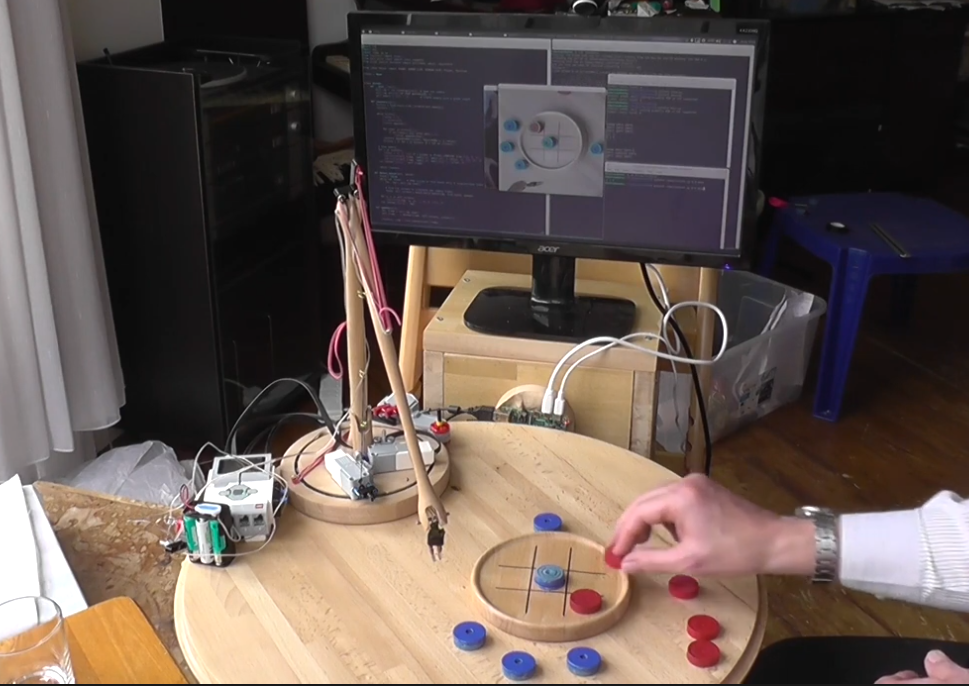
\includegraphics[scale=0.3]{robot.png}
    \caption{Screenshot of the robot in play.  Longer video can be seen at https://www.youtube.com/watch?v=f7gmhgkUHVI}
\label{fig:robot}
\end{figure}

To briefly add to the motivation of this project it's worth noting a robotic arm and vision system I have built that can successfully play board games.
It was found that in building such a system, one of the hardest things to get right was the vision system.  As can be seen, this robot arm is 
made of wood, Lego, strings, elastic band and still is able to play a full game through.
Unfortunately this vision system only works with board games with two counters, specifically circular counters that work well with the 
Hough transform.  
The goal, is to build a vision system that would spark the creation of a robot that can play chess with you.
In this journey to build such a system, I knew neural networks would be necessary, and I thought I had a good chance at beating the existing solutions
out there by leveraging the amazing work that has come out of the deep learning community.
But first, it was important for me to understand the fundamentals so I built an automatic differentiation library, similar to that of pytorch which can be
viewed on github (https://github.com/Mulac/autograd-light).
